\subsection{Persistence under a transverse perturbation}\label{sec:unfolding}
The algebraic boundary of the balanced example is not destroyed by a small
asymmetry of the fast hidden state's exits.  Define $Q(z,\delta)$ from
Eq.~\eqref{eq:theta} by replacing its last row with
\begin{equation}
 (z+\delta,z-\delta,0,0,-2z),\qquad z>|\delta|.
\end{equation}
The hidden pole locations and output wedge remain fixed as $\delta$ varies;
the fast-pole input residue changes.  This perturbation is neither a time
rescaling nor a hidden permutation.

\begin{proposition}[Local persistence of the feasibility transition]\label{prop:unfolding}
In the reciprocal irreducible class with at most five states, there is a
smooth critical curve $z_*(\delta)$ through $(\zs,0)$.  In a neighborhood of
that point the compatible entropy fiber is unbounded for $z<z_*(\delta)$,
has exactly two distinct finite values at $z=z_*(\delta)$, and has a unique
generator for $z>z_*(\delta)$, up to hidden permutations.  The curve satisfies
\begin{align}
 \mathcal P_\delta(z)={}&\mathcal P(z)-(20160z+14112)\delta\nonumber\\
 &-(352z^2-3168z+15768)\delta^2=0,\label{eq:perturbedP}\\
 z_*'(0)={}&\frac{20160\zs+14112}{\mathcal P'(\zs)}
 \simeq0.4650042.\label{eq:perturbedslope}
\end{align}
This is a local statement for the specified perturbation, not a generic
classification of five-state networks.
\end{proposition}

\begin{proof}[Proof structure] Appendix~\ref{app:unfolding} proves the perturbed discriminant identity, certifies the strict support-exhaustion and construction margins on a rational rectangle, and transfers the unique-equality and subcritical opening arguments. The entropy gap persists locally by the balanced exact certificate and continuity on fixed positive supports.\end{proof}



The reduced boundary equation has the exact normal form
\begin{equation}
 F(t;z,\delta)=f_2(t-t_c)^2-\frac{\Delta}{4f_2},
 \qquad t_c=-\frac{f_1}{2f_2},\quad f_2<0.\label{eq:foldnormal}
\end{equation}
Its two active-boundary path roots merge with square-root scaling as
$\Delta\downarrow0$.  This is a nondegenerate fold of the boundary
equation.  The full feasible set has a complete-realization continuum
below the curve and the source persists on both sides; it is therefore
not a saddle-node of two isolated positive realizations.  No conclusion
about arbitrary perturbations of the source rates or hidden dimension
follows from this one unfolding.

\begin{figure*}[t]
 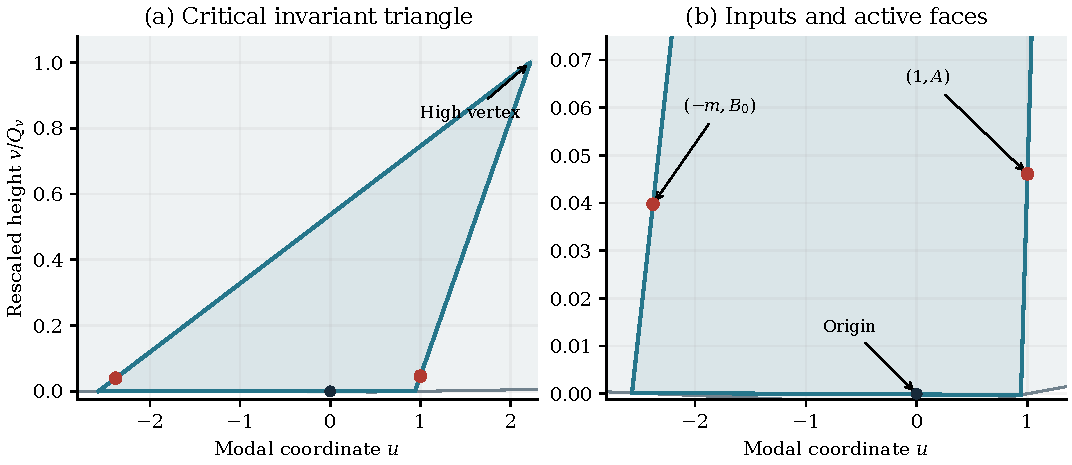
\includegraphics[width=\textwidth]{figures/realization-geometry.pdf}
 \caption{Geometry at the critical balanced parameter.  The invariant
 triangle lies inside the output wedge and contains the two input points
 (red).  The vertical coordinate has been rescaled by its maximum vertex
 height; this invertible rescaling preserves incidences and invariance.
 Panel (b) enlarges the input region.  Active input, output and tangent
 constraints determine the reciprocal path realization.}
 \label{fig:realizationgeometry}
\end{figure*}

\begin{figure*}[t]
 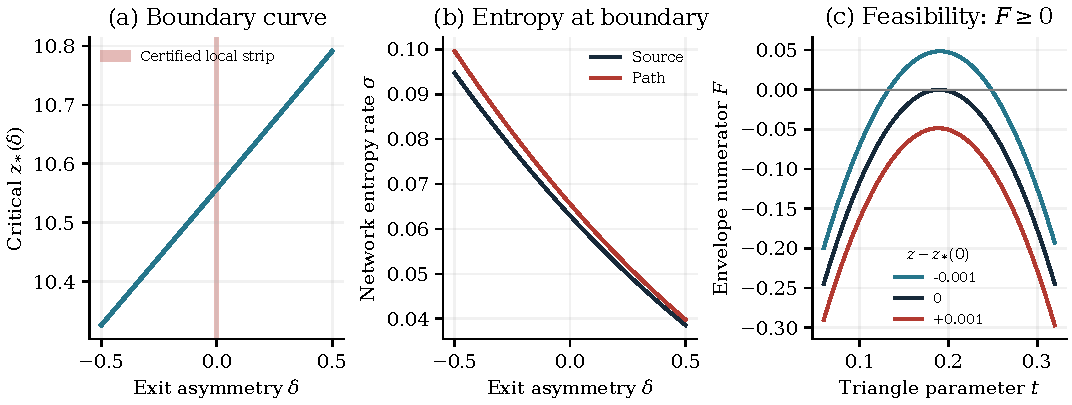
\includegraphics[width=\textwidth]{figures/continuation.pdf}
 \caption{Specified exit-asymmetry unfolding.  (a) Numerical continuation
 of the boundary over $-0.5\le\delta\le0.5$; the narrow highlighted strip
 is the range with the exact geometric certificate~\eqref{eq:unfoldrect}.
 (b) Source and path entropy at the numerical boundary.
 (c) The envelope numerator is nonnegative precisely between its two
 boundary roots below the critical parameter.  The wider curves are
 numerical diagnostics, not global off-balanced support exhaustion.}
 \label{fig:continuation}
\end{figure*}

The deterministic continuation uses 41 $\delta$ nodes at spacing $0.025$,
80-digit arithmetic, and offsets $z-z_*(\delta)=\pm0.001$.  At all these
nodes it finds two, one, and zero admissible \emph{active-boundary path
candidates} below, at, and above the curve.  These are not counts of all
positive realizations outside the proved rectangle.  Complete positive
realizations are separately constructed below each node.  The generator
orbit Jacobian has numerical rank six, whereas the six active-zero
constraint Jacobian has rank six on either path branch and rank five at
their merger, using relative singular-value tolerance $10^{-10}$.
Present critical rates remain above $0.1645$ in this grid.  Structural
zeros are checked below $10^{-65}$ without clipping; exact all-time
equality comes from the modal similarity identity.  Independent
120-digit recomputation at $\delta=-0.5,0,0.5$, direct matrix-exponential
checks, and the historical exact path-witness comparison are recorded
with source hashes, commands, precision and all numerical outputs.
